\section{Approach}
\label{sec:approach}
We propose \hl{3 or 4} time series transformers of different architectures to forecast proton intensities from preceding relativistic electrons. We use a window of electron and proton intensities to make predictions. Current transformer models have been appealing as to researchers as they have the ability to capture long range dependencies and scale effectively with large dataset. This makes them suitable  for our challenge of  time series forecasting with multi horizon demand predictions.\cite{zhao2026transformersurvey}. We make a selection of transformer models of different architectures to model our incoming proton intensity flux. 

Section \ref{sec:input} will discuss the time time series datas and characteristics. Section \ref{sec:m1transformer} outline our transformer approach and compare the architectures with \cite{torres2025machine}. In Section \ref{sec:positionalencodingmethods}, we will explain each of the used archtiectures in our study.

\subsection{Input}
\label{sec:input}

\begin{figure}[!htbp]
    \centering
    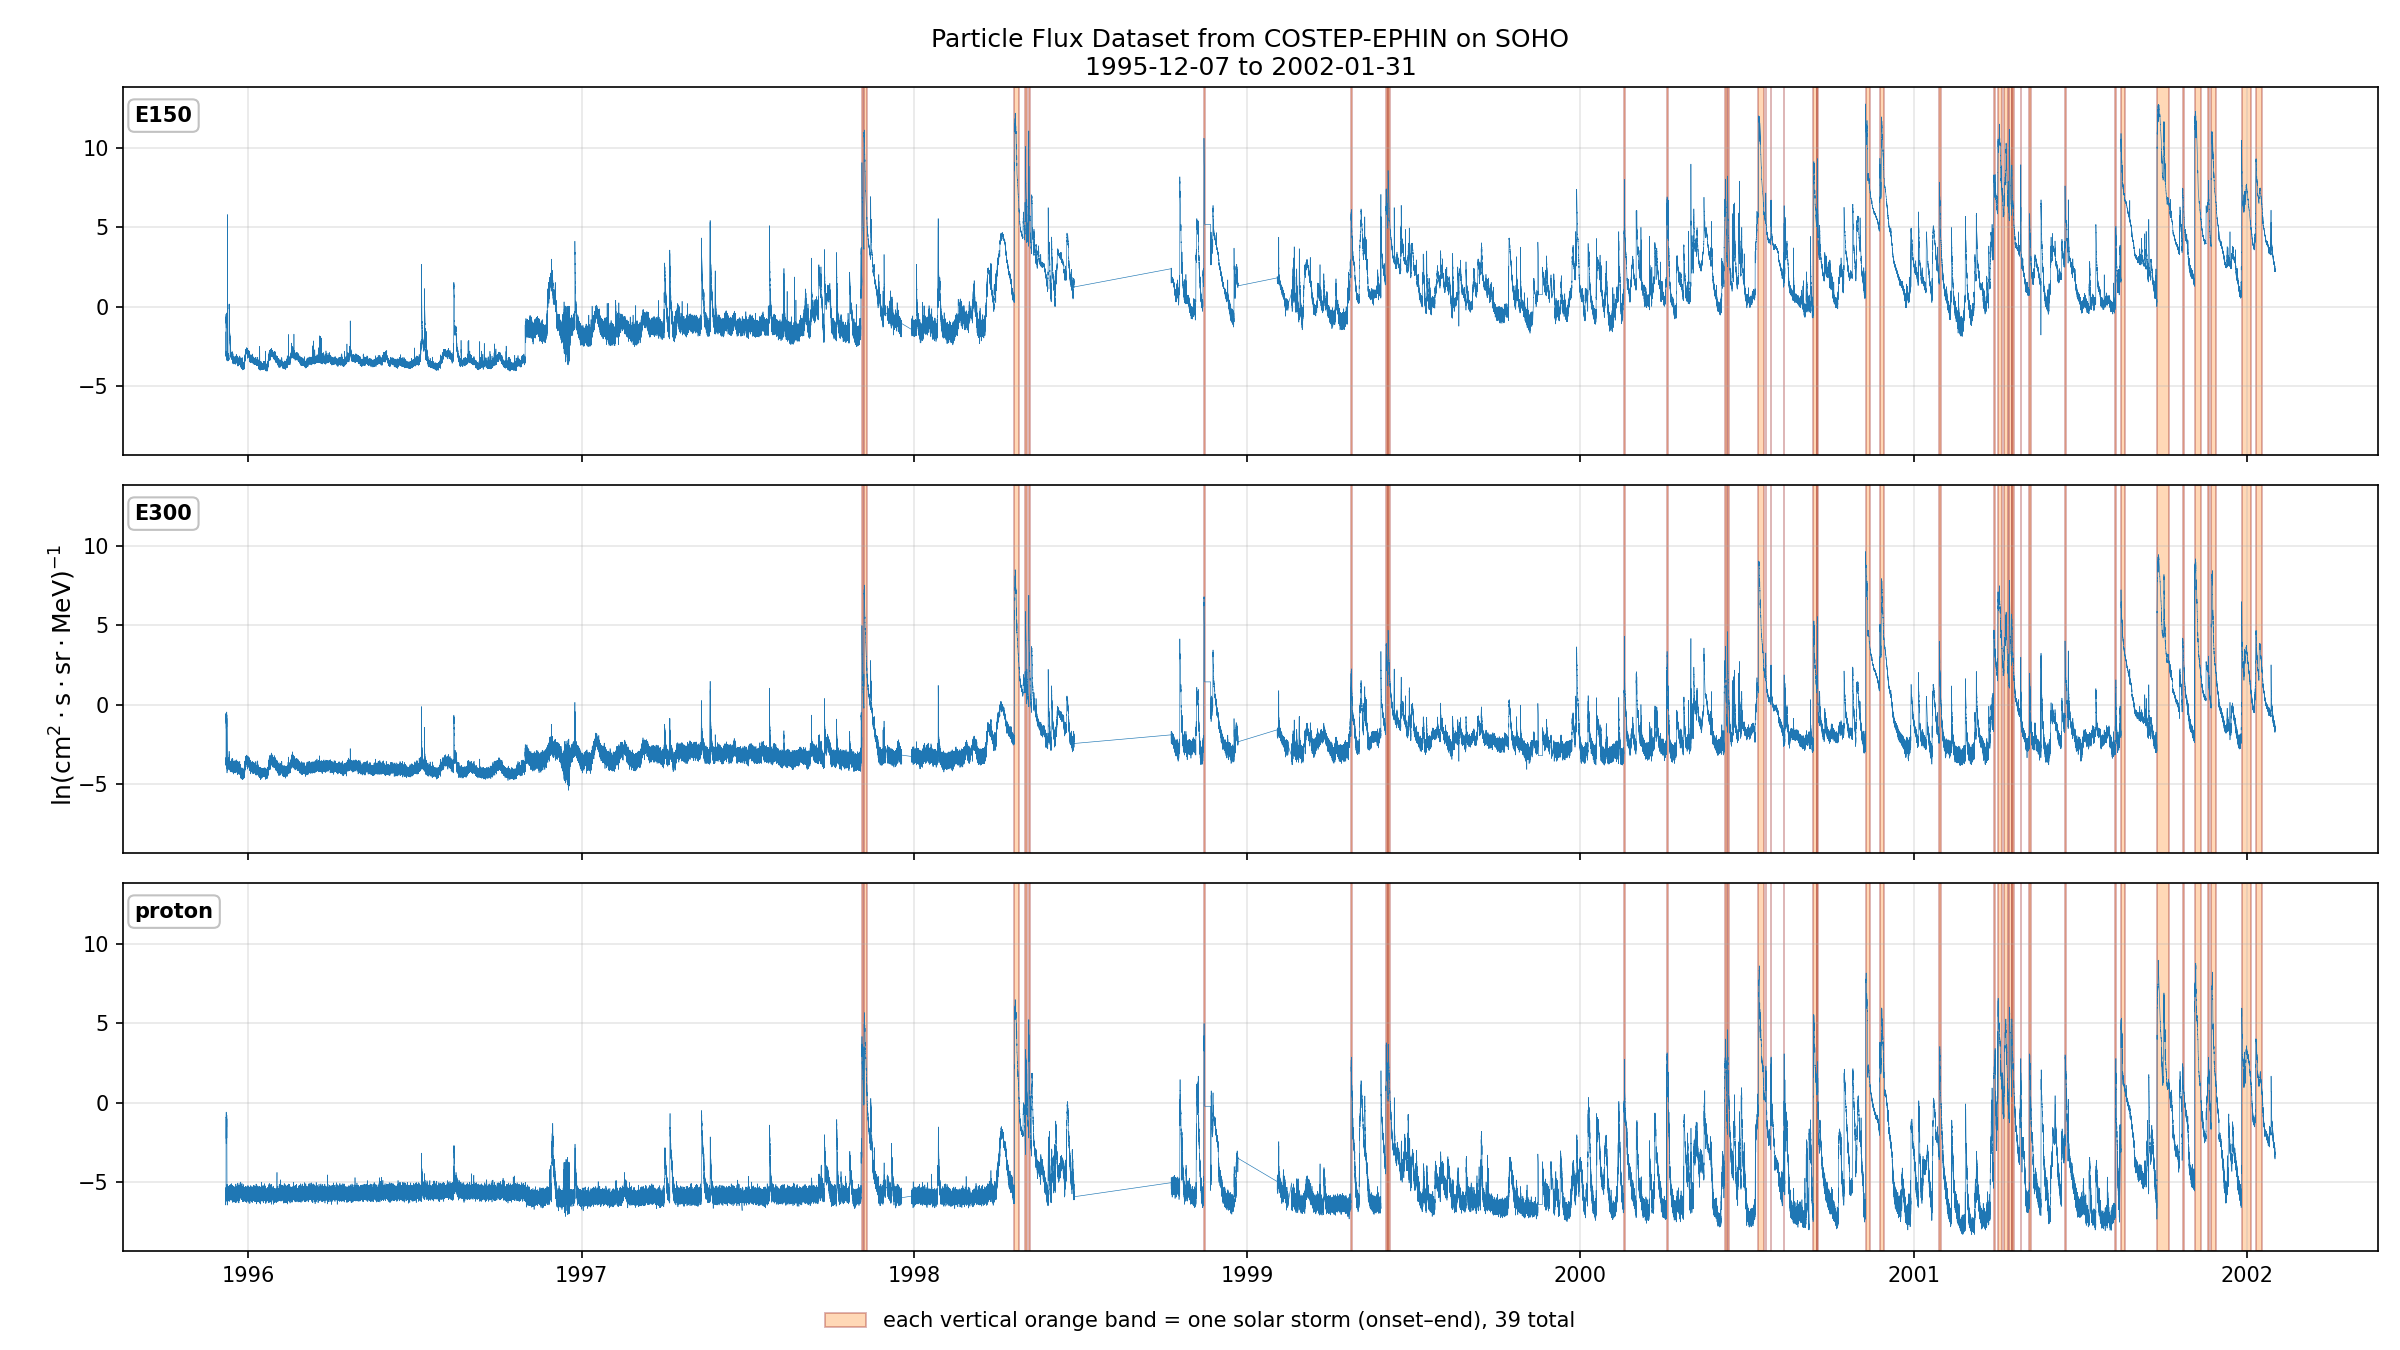
\includegraphics[scale=.40]{plots/data_overview.png}
    \caption{SOHO COSTEP-EPHIN dataset from 1995-2002}
    \label{fig:sinusoidal_t6_comparison}
\end{figure}

\begin{figure}[!htbp]
    \centering
    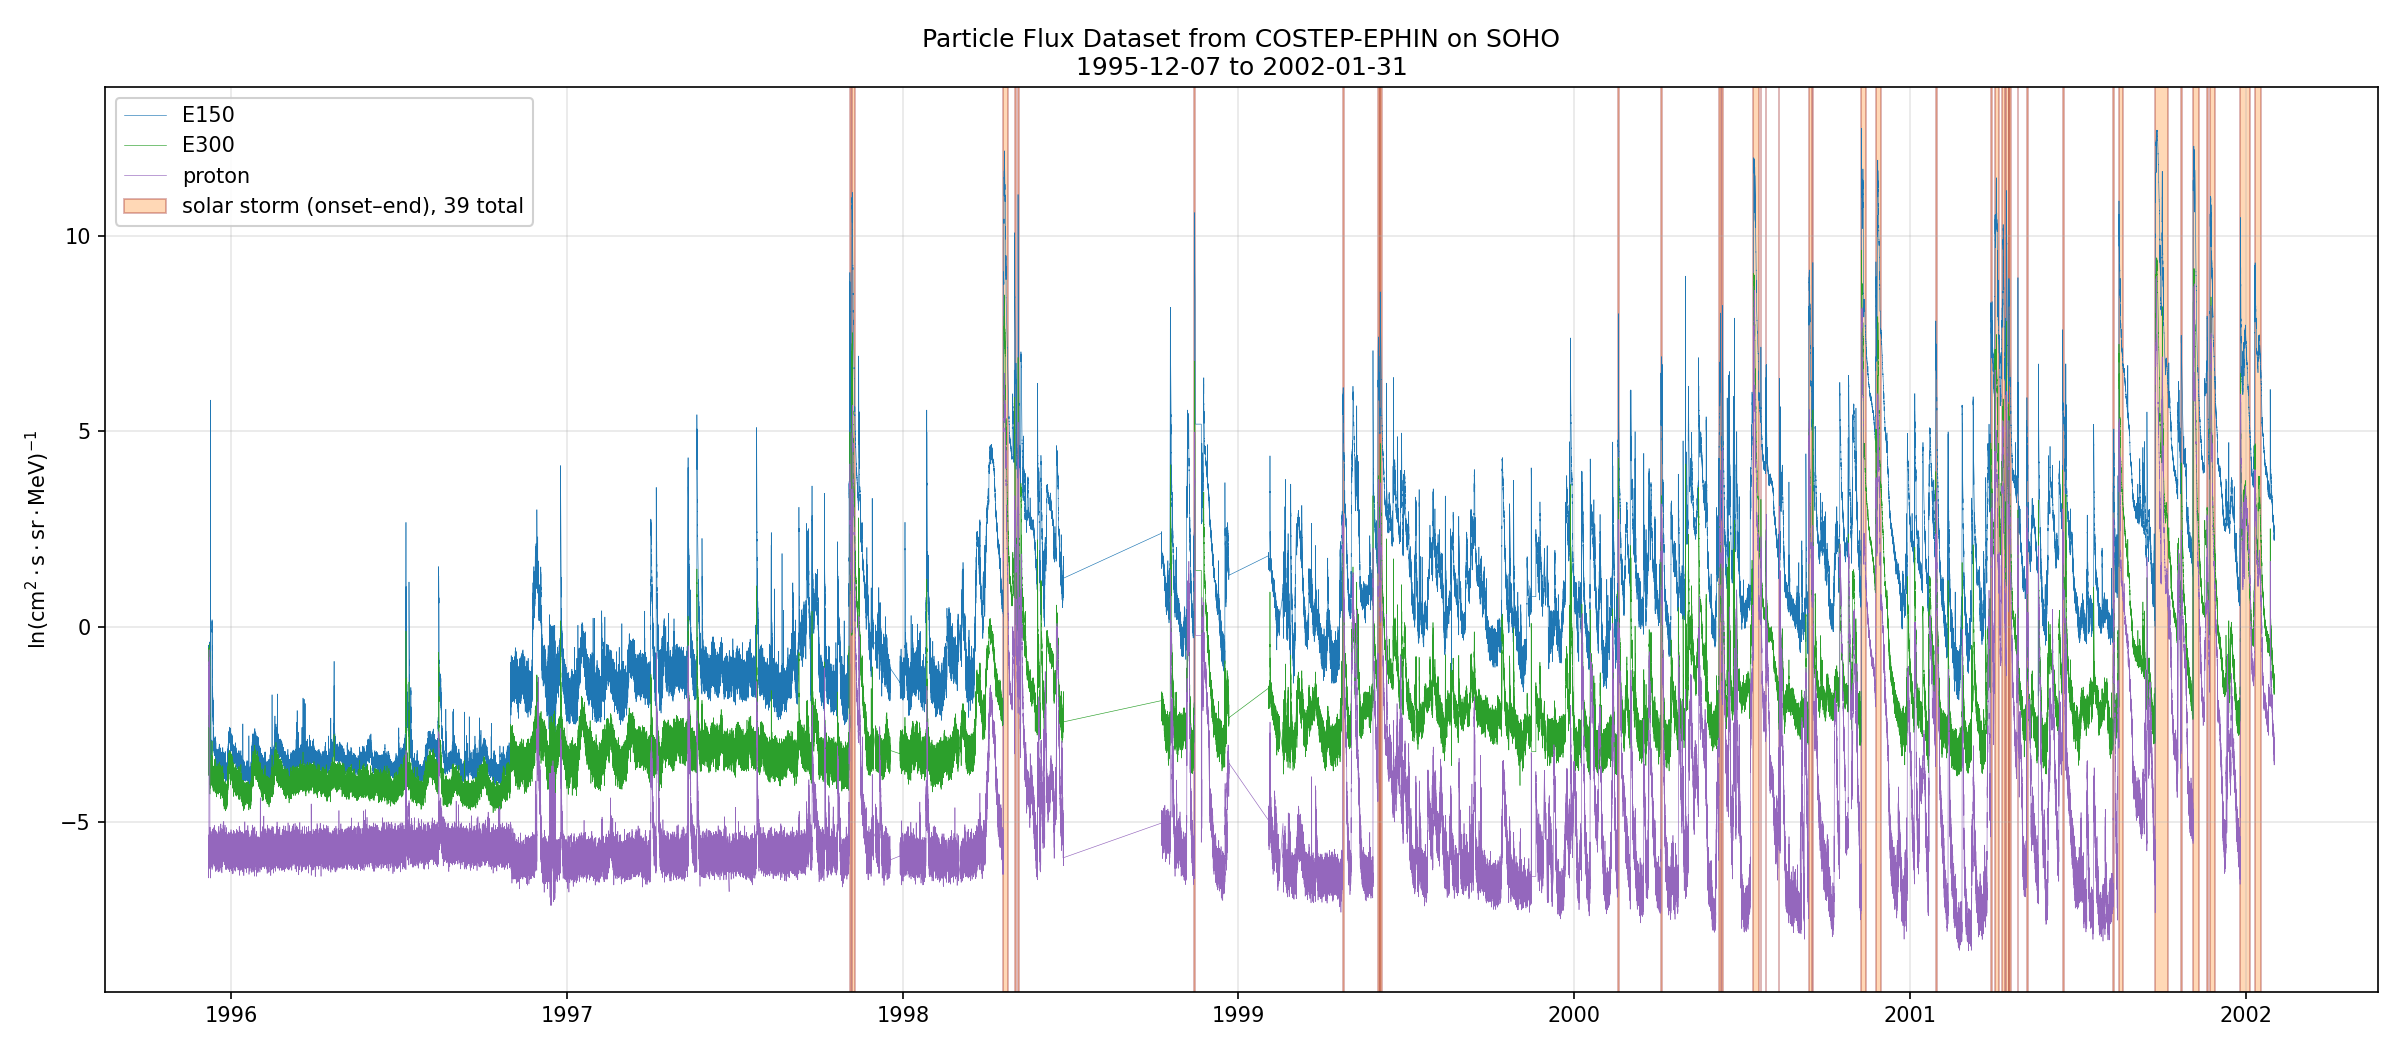
\includegraphics[scale=.40]{plots/data_overview_single.png}
    \caption{SOHO COSTEP-EPHIN dataset from 1995-2002}
    \label{fig:sinusoidal_t6_comparison}
\end{figure}

The input data  is obtained from the Comprehensive Suprathermal and Energetic Particle Analyzer - Electron Proton Helium Instrument (COSTEP-EPHIN)  on the Solar and Heliospheric Observatory (SOHO) located at Lagrange Point 1 (L1). The main features we will be using to make are proton flux predictions are two electron intensities channels $\geq$0.25 and $\geq$0.67 MeV and the current proton intensity channel $\geq$10 MeV \cite{mullermellin1995costep}. In total, the number of timestamped fluxes is $\approx 600,000$ entries. The resultant proton channel has been integrated across several channels (P4, P8, P25, P41) and interpolated using the power-law spectrum. A peak detection algorithm then sliced each SEP event for storms larger than 10 pfu and timestamped each phase within storm: Onset, threshold, peak, and end. The onset is defined when the flux rises three times the error bar above the pre-event background, the threshold is when the flux first crosses over 10 pfu and the end time is when it drops again below 2 pfu.\cite{torres2025machine}. Each timestamp in our event catalogue is given a bool idicating which phase the flux is in. The proton flux projections are calculated by a 2 hour window of the two electron channels and the proton fluxes and then casted out by both 30 minutes $(t+6)$ and 1 hour $(t+12)$.

\subsection{M1 Transformer}
\label{sec:m1transformer}
We name our transfomer "M1 Transformer" after the M1 RNN in \cite{torres2025machine}. RNNs are unreliable for long range forecasting and irregular patterns \cite{zhao2026transformersurvey}. This is prevalent in our particle flux data with long periods of noise with sudden spikes when a storm occurs. Transformers are able to capture these long patterns of behavior with improved predictions with parallel processing while RNNs process only in series. The Transformer attention mechanism is able to analyze all time steps at once and focus on relevant steps regardless of order \cite{vaswani2017attention}.  This method of parallel analytical processing reveals subtle patterns that would be overlooked by RNNs \cite{zhao2026transformersurvey}. Our transformer will only have an encoding only architecture as we are forecasting one value of proton flux, therefore a single output layer is required only. If we were to predict a series proton fluxes then a decoder would be required.

\begin{figure}[H]
    \centering
    \resizebox{0.6\textwidth}{!}{
    \begin{tikzpicture}[
        pebox/.style={
            draw, rounded corners=2pt, fill=green!25,
            minimum width=2cm, minimum height=1cm, thick,
        },
        mhbox/.style={
            draw, rounded corners=2pt, fill=red!25,
            minimum width=3cm, minimum height=1.5cm, thick,
        },
        normbox/.style={
            draw, rounded corners=2pt, fill=orange!25,
            minimum width=3.0cm, minimum height=.5cm, thick,
        },
        feedforwardbox/.style={
            draw, rounded corners=2pt, fill=violet!25,
            minimum width=3.0cm, minimum height=1.5cm, thick,
        },
        linearbox/.style={
            draw, rounded corners=2pt, fill=yellow!25,
            minimum width=3.5cm, minimum height=.5cm, thick,
        },
        softmaxbox/.style={
            draw, rounded corners=2pt, fill=teal!25,
            minimum width=3.5cm, minimum height=.5cm, thick,
        },
        scale = 1
    ]

        % outer container: the whole encoder block


        \node (pe) at (0,-8) {$\bigoplus$};
        \node[
            draw,
            rounded corners=15pt,
            fill=gray!25,
            minimum width=6cm,
            minimum height=8.5cm,
            thick,
            above = 20mm of pe,
        ] (outer){};

        % positional-encoding options, stacked left of pe: RoPE level with pe,
        % Sinusoidal/Zero-Init symmetric above/below it -- no manual coordinates
        
        \node[text= olive, text width = 3 cm, align=center](pe_disclaimer) at (-6,-6){Only one of the positoinal enoders (RoPE, Sin, Zero) are used for each training run }
        \node[pebox, above left =.5mm and 2cm of pe] (Sinusoidal) {Sinusoidal};
        \node[pebox, below left =.5mm and 2cm of pe] (Zero-Init) {Zero-Init};
        \node[mhbox, above=35mm of pe, text width = 2 cm, align=center] (MultiHead) {Multi-Head Attention};
        \node[normbox, above = 1.5 cm of MultiHead] (norm1){Norm};
        \node[pebox, left=2cm of MultiHead] (RoPE) {RoPE};
        \node[
            draw, rounded corners=5pt, fill=blue!25,
            minimum width=2cm, minimum height=1cm, thick,
            below=10mm of pe,
        ] (Input_Embedding) {Input Embedding};
        \node[feedforwardbox, above =  5mm of norm1, text width = 2 cm, align=center](FeedForward){Feed Forward};
        \node[below= 1cm of Input_Embedding, text width = 3cm, align=center](input) {2 hour window of high and low electrons w/ current proton flux};
        \node[normbox, below = 2cm of MultiHead](norm2){Norm};


        \node[align = center] at (-5,-2){$\times 1$ Encoding Layers};
        \node[above = 5mm of MultiHead] (pe2) {$\bigoplus$};
        \node[above = 5mm of FeedForward] (pe3) {$\bigoplus$};
        \node (pe) at (0,-8) {$\bigoplus$};
        \node[linearbox, above = 8mm of pe3](linear){Linear};

        \draw[->,thick](input.north) -- (Input_Embedding.south);
        \draw[->, thick, rounded corners=5pt] (Input_Embedding.north) -- (pe.south);
        \draw[->, thick, rounded corners=5pt] (RoPE.east) -- (MultiHead.west);
        \draw[->, thick, rounded corners=5pt] (Zero-Init.east) -| ++(5mm,8.55mm) -- (pe.west);
        \draw[->, thick, rounded corners=5pt] (Sinusoidal.east) -| ++(5mm,-8.55mm) -- (pe.west);
        \draw[->, thick, rounded corners=5pt] (pe.east) -| ++(15mm,0) |- (pe2.east);
        \draw[->, thick, rounded corners=5pt] (pe2.east) -| ++(15mm,0) |- (pe3.east);
        \draw[->, thick, rounded corners=5pt] (norm2.north) |- ++(-7mm,15mm) -| ($(MultiHead.south west) + (5mm,0)$);
        \draw[->, thick, rounded corners=5pt] (norm2.north) |- ++(7mm,15mm) -| ($(MultiHead.south east) - (5mm,0)$);
        \draw[->, thick] (norm2.north)  -- (MultiHead.south);
        \draw[->, thick] (pe.north)  -- (norm2.south);
        \draw[->,thick](norm1.north) -- (FeedForward.south);
        \draw[->,thick](FeedForward.north) -- (pe3.south);
        \draw[->, thick](pe3.north) -- (linear.south);
        \draw[->, thick , rounded corners=5pt]($(pe)!0.60!(MultiHead)$) -| ++(-25mm, 15mm) |- (norm1.west);
        \draw[->,thick](MultiHead.north)--(pe2.south);
        \draw[->, thick](pe2.north)--(norm1.south);
        \draw[->,thick, text width = 3 cm, align=center](linear.north) -- ++(0,5mm) node[above] {Forecasted proton flux at $t+6$/$t+12$};
        \path (5,-2); % invisible point, balances the bounding box against the "$\times 1$" label on the left
    \end{tikzpicture}
    }
    \caption{M1- Transformer Architecture with positional encodings}
    
    \label{fig:transformer-pe}
\end{figure}


We must ensure that the total number of parameters of our transformer models (Sinusoidal,  RoPE, T5, Zero Init)  approximate to Torres's RNN's and NN's total number of parameters. Both the RNN and NN are implemented using Keras in python consisting of two layers: One layer is hidden with 30 units and then a second dense single output layer. The RNN is comprised of  Gated Recurrent Units (GRU) for its  hidden layers while the NN uses hidden layers. The NN model uses the same three channels for 25 timestep intervals. The RNN  has the 30 GRU units plus our three channel input \cite{torres2025machine}. 



\begin{figure}[!htbp]
\centering
\begin{tikzpicture}
\matrix (tbl) [
    matrix of nodes,
    nodes={draw, minimum width=3cm, minimum height=0.8cm, anchor=center},
    row sep=-\pgflinewidth,   % rows/cols share borders instead of doubling them
    column sep=-\pgflinewidth,
    column 1/.style={nodes={font=\bfseries}},   % bold first column
    row 1/.style={nodes={font=\bfseries, fill=gray!20}}  % shaded header row
]
{
    Models              & Parameters \\
    NN    & 2,311       \\
    RNN     & 3,181       \\
    Sinusoidal     & 3,361       \\
    Zero Init   & 3,761 \\
    RoPE   & 3,361 \\
};
\end{tikzpicture}
\caption{Model type and their number of total parameters}
\label{fig:param-table-template}
\end{figure}

The $+2$ in the RNN calculation is to reflect Keras' $\texttt{reset\_after = True}$ GRU parameterization

\subsection{Positional Encoding Methods}
\label{sec:positionalencodingmethods}
RNN models read in data sequentially as they train, learning order inherently. Transformers, however, lack this ability due to parallelization in the processing and require positional encoding methods to order the tokens. In this study, we will be showcasing four positional encoding methods to forecast our SEP events: Sinusoidal, Rotary Positional Encoding (RoPE), Zero-Init. These approaches injections the positional information differently and results in varied SEP prediction accuracy.

\subsubsection{Sinusoidal Positional Encoding}
Sinusoidal positional encoding was first introduced in the original proposed transformer architecture paper \cite{vaswani2017attention}. It is an absolute position encoding method that uses $\sin$ and $\cos$ functions of different frequencies to encode the positional indexes of tokens in a sequence. For each token, a vector of dimension \texttt{dim\_val} is given. each token vector is determined by the position they are in, in a sequence and the length of the vector.  Odd and even indexes in the vector are determined by \eqref{cosPE} and \eqref{sinPE} respectively. Both \eqref{cosPE} and \eqref{sinPE} are used rather than just \eqref{sinPE} is because we can represent a linear relationship between two encoded positions. Once these tokens have their positional indexes the attention block computes their own QKV matrices allowing for predictions to occur.

\begin{equation}
    \label{sinPE}
   PE_{(pos,2i)} = \sin (pos / 10000^{2i/d_{model}}) 
\end{equation}

\begin{equation}
    \label{cosPE}
   PE_{(pos,2i+1)} = \cos(pos/10000^{2i/d_{model}})
\end{equation}

 The frequency of the $\sin$ and $\cos$ functions decreases exponentially by a scale factor as the position in the model dimensions increase. For short term we can find fine grain details in data, a $\sin/\cos$ function with a high frequency. At large vector indexes the frequency greatly decreases, taking on a more linear relationship. The sin and cos functions keep all values tokenized values within a range of [-1,1] which is easy for the transformer to understand eliminating the need for standardization. The positions are encoded uniquely based on value and position, allowing it to scale to unlimited sequence lengths. 



\subsubsection{Rotary Positional Embedding}
Rotary Positional Embedding (RoPE) is a relative positional embedding method that encodes the  relative positions of embedded vectors to the dot product of two rotated vectors. The rotation of the vectors is determined by their order in the sequence. The relative positions are then used for self attention formulation \cite{su2021roformer}. The rotated embedded vector is the product of the rotation matrix, query-key weight matrix and our input vector:
\begin{equation}
    f_{\{q,k\}}(\mathbf{x}_m, m) = 
    \begin{pmatrix} 
    \cos m\theta & -\sin m \theta  \\
    \sin m\theta & \cos m\theta 
    \end{pmatrix}
    \begin{pmatrix} 
    W_{\{q,k\}}^{(11)} & W_{\{q,k\}}^{(12)}  \\ W_{\{q,k\}}^{(21)} & W_{\{q,k\}}^{(22)} 
    \end{pmatrix} 
    \begin{pmatrix} 
    x_m^{(1)}\\
    x_m^{(2)}
    \end{pmatrix} 
\end{equation}
in 2D coordinates. A simple rotation of the word embedding vector by an angle multiple of its position index is the main idea behind Rotary Position Embedding \cite{su2021roformer}.

A property of RoPE is long term decay. This means that pairs of tokens at large relative distance will have less connection than those that are close to each other \cite{su2021roformer}. For our flux data, this would coincide with the idea from \cite{posner2007forecasting} that only a short term forecasting of relativistic electrons is required to accurately predict future proton storms from 30 minutes to an hour. 


\subsubsection{Zero-Initialized}
Zero-Initialized positional encoding is an absolute positional that sets all  positional encoding parameters in a transformer to zero at the start of training This means that positon of a timestamped flux has equal effects on each other at the start. then as training continues, near timestamped fluxes learn to correlate to each other rather than further ones. With a zero or near zero initialization, models on their own learn patterns that are used to make predictions with zero valued starting weights. Zero init contrast Sinusoidal who all have non zero starting weight values. RoPE does not have positional parameters rather computes weights analytically. This makes it reliable for generalization which is ideal for SEP data made almost entirely of background fluxes \cite{torres2025machine}. Commonly, small near zero initializations sampled with normal distributions were found to perform better than larger ones \cite{ito2024learning}.
% \begin{equation}
% \label{normalDistWeight}
%     \mathscr{N} ( \mathbf{0}, \mathbf{\Sigma}), \mathbf{\Sigma} = \sigma\mathbf{I}
% \end{equation}
% \begin{equation}
%     \label{sigmaWeightZero}
%     \sigma \in \left\{ 0 \right\}
% \end{equation}

Most timestamps in the relatively small proton electron flux dataset are near zero background values. A larger starting weights already has background information included leading to forecasting more background in the future during the early portion of training. Its not until after rounds of epochs to unlearn patterns are to finally map where spikes in fluxes start to occur in order to make accurate predictions.
